% Chapter 3: Realisation and tests. Firmware sections are written from the code on main
% (firmware as restructured 2026-10-25: src/*.cpp and include/*.h of the robot, Bloc-Con/src and Bloc-Con/include of the controller).

\chapter{Realisation and tests}
\label{ch:realisation}

\section{Introduction}
Chapter~\ref{ch:design} chose the components and explained how each one works. This
chapter describes how they were put together: the wiring of the two boards, the firmware
that runs on them, the problems met along the way and how they were solved, and the tests
that show what the finished system does. It ends with the cost of the platform.

\section{Wiring}
\label{sec:wiring}
Both boards are built from ready-made modules connected with jumper wires, so their
schematics are drawn at module level, in KiCad: each module appears as a box carrying
the pins of its header, and connections are made by giving the same net name to the pins
that are joined, a common convention that keeps a schematic readable when many wires
would cross. Only the microcontroller pins in use are shown. The robot's schematic is
given in Figure~\ref{fig:sch-robot} and the controller's in Figure~\ref{fig:sch-con}; their
pin assignments are those of Tables~\ref{tab:robot-pins} and~\ref{tab:con-pins}. KiCad's
electrical rules check reports no unconnected pin or dangling net on either sheet.

Three points of the robot's wiring deserve a comment. The DRV8833's \texttt{STBY} pin is
tied to 3.3~V, so the driver is always enabled and no GPIO is spent on it, and its three
NC pins, kept from the TB6612FNG board layout, are left open. The right motor's inputs
are wired to GPIO~17 and~18 in that order but swapped in the firmware, so that both
wheels turn forward for the same command; changing two constants was simpler than
rewiring. Finally, the HC-SR04's \texttt{ECHO} line reaches GPIO~12 through the
1~k\(\Omega\)/2~k\(\Omega\) divider of Section~\ref{sec:hcsr04}.

On the controller, the cell is connected to the battery terminals (B+, B$-$) of the
TP4056 module and everything else to its protected output (OUT+, OUT$-$), so the
protection of Section~\ref{sec:con-power} covers the whole controller. The power switch
sits between that output and the MT3608, and the four buttons go straight from their GPIO
to ground.

\begin{sidewaysfigure}
  \centering
  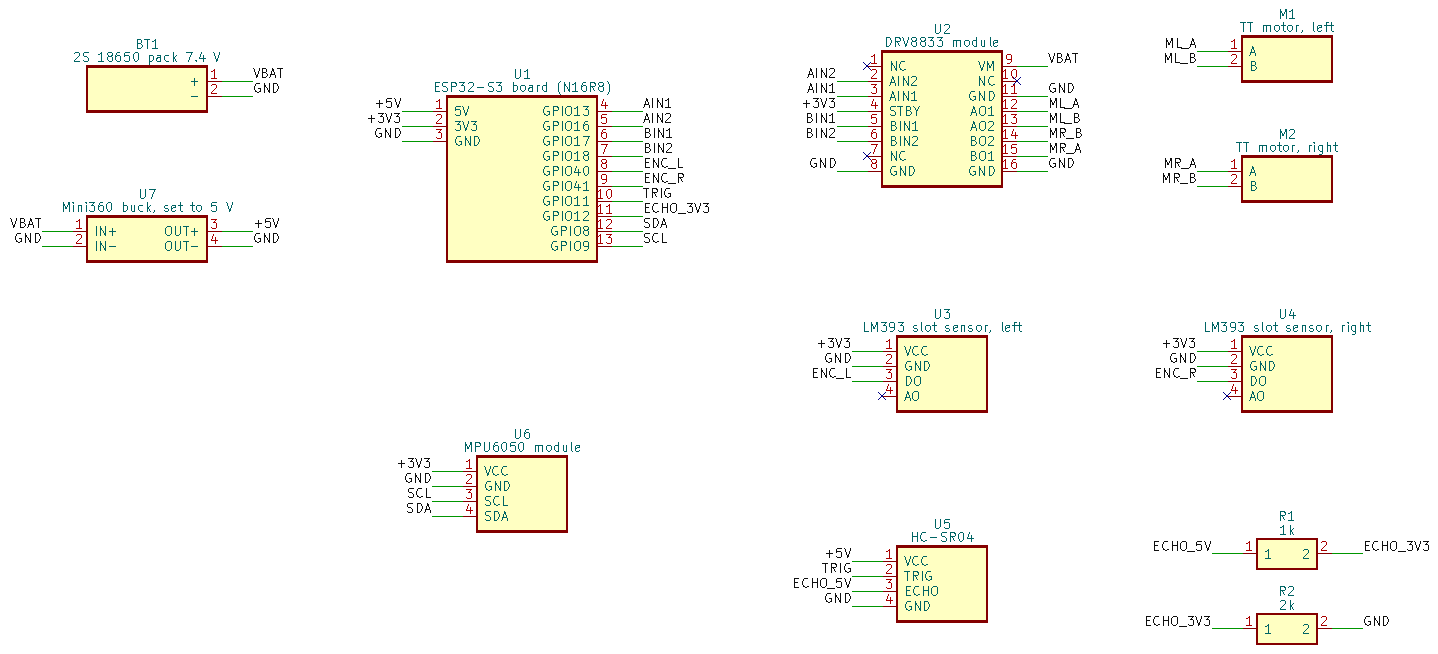
\includegraphics[width=\textheight]{../circuits/kicad/robot/robot.pdf}
  \caption{Schematic of the robot, drawn in KiCad. Modules are drawn as boxes with their
           header pins; pins carrying the same net name are connected. Only the
           ESP32-S3 pins in use are shown. Not shown: the main switch, a BMS and a fuse,
           which are not fitted yet.}
  \label{fig:sch-robot}
\end{sidewaysfigure}

\begin{sidewaysfigure}
  \centering
  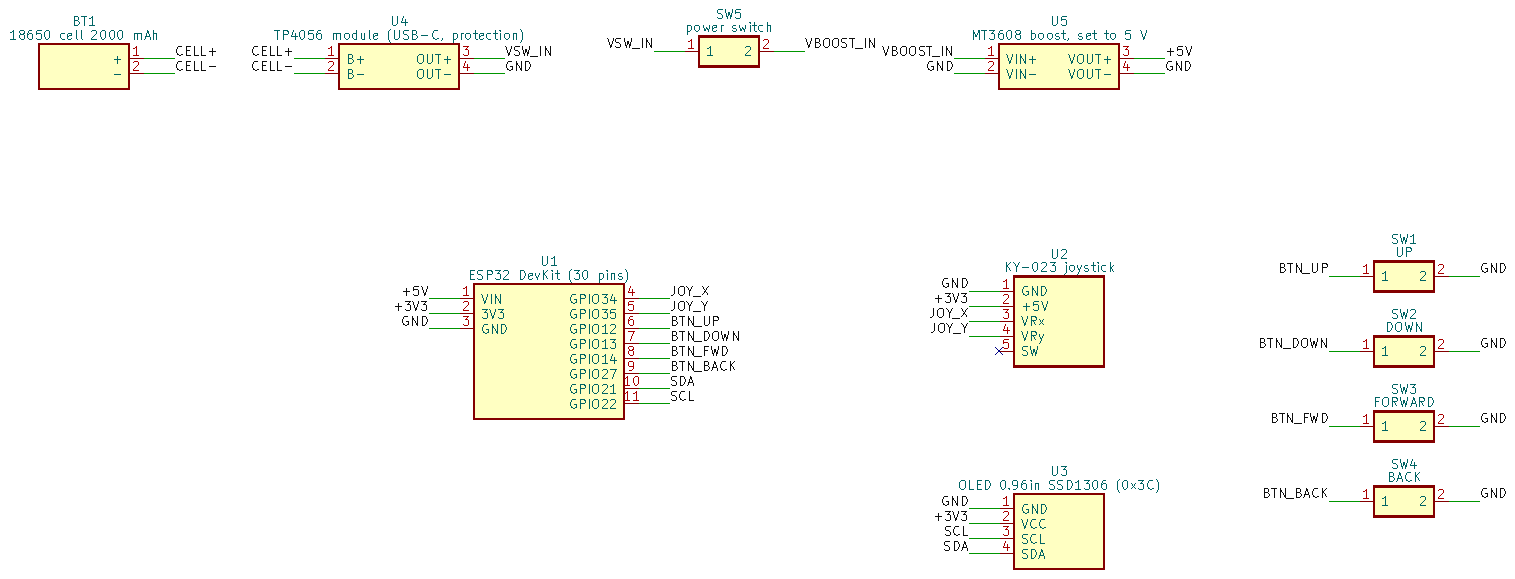
\includegraphics[width=\textheight]{../circuits/kicad/controller/controller.pdf}
  \caption{Schematic of the controller, drawn in KiCad, with the same conventions as
           Figure~\ref{fig:sch-robot}. The joystick is powered from 3.3~V although its
           pin is labelled +5V. The HC-SR04 wired to the controller during bench tests is
           not shown, since the sensor now sits on the robot.}
  \label{fig:sch-con}
\end{sidewaysfigure}

\plan{Photos of the wired robot and controller. \todo{photos}}

\section{Firmware}
\label{sec:firmware}

\subsection{Tools}
Both boards are programmed in C++ with the Arduino framework for Espressif chips, inside
PlatformIO, an open build system that fetches the toolchain and the libraries a project
declares and builds and uploads the firmware. Each board has its own project: the robot's
at the root of the repository, the controller's in \texttt{Bloc-Con}. The controller
also uses the U8g2 graphics library to drive its display. All the source code is kept in
a single Git repository, whose history is also the record of what was changed and when.
The firmware is built with PlatformIO Core 6.1.19, its Espressif~32 platform 7.1.2
and version 2.0.17 of the Arduino core for ESP32. The controller's firmware was also run in
Wokwi, an online simulator for microcontroller boards, before it was loaded on the real
board. The simulated circuit, kept in the project as \texttt{diagram.json}, contains an
ESP32 board, an SSD1306 display, an analogue joystick, the four push buttons and an
HC-SR04, so the menus and screens could be tried without the hardware.

The code of each board is split into one file per function, listed in
Table~\ref{tab:modules}, so that each part can be read, tested and changed on its own.
The packet formats are defined in a single header, \texttt{packets.h}, kept identical in
both projects so that the two ends always agree on them.

\begin{table}[htbp]
  \centering
  \caption{Organisation of the firmware (\texttt{.cpp} file and its \texttt{.h} header).}
  \label{tab:modules}
  \begin{tabularx}{\textwidth}{@{}l X@{}}
    \toprule
    File & Role \\
    \midrule
    \multicolumn{2}{@{}l}{\textit{Robot}} \\
    \texttt{main} & start-up and the 10~ms main loop \\
    \texttt{radio} & ESP-NOW set-up, sending, reception callback \\
    \texttt{drive} & drive commands: reception, mixing, link indicator \\
    \texttt{motor} & PWM output, soft start, failsafe \\
    \texttt{encoders} & wheel-speed measurement \\
    \texttt{ultrasonic} & HC-SR04, echo timed by interrupt \\
    \texttt{imu} & MPU6050 and the complementary filter \\
    \texttt{bench} & serial commands for bench tests \\
    \texttt{pins\_esp32s3.h} & pin assignment \\
    \midrule
    \multicolumn{2}{@{}l}{\textit{Controller}} \\
    \texttt{main} & start-up and the main loop \\
    \texttt{radio} & ESP-NOW set-up, drive commands, data received from the robot \\
    \texttt{joystick} & calibration and reading \\
    \texttt{ui} & buttons, menu, splash, About and Settings screens \\
    \texttt{screen\_drive}, \texttt{screen\_ultrasonic}, \texttt{screen\_mpu} & one file
      per screen \\
    \texttt{display}, \texttt{config.h} & display object, pin assignment \\
    \midrule
    \texttt{packets.h} & packet formats, shared by both projects \\
    \bottomrule
  \end{tabularx}
\end{table}

\subsection{Communication protocol}
\label{sec:protocol}
The two boards exchange four kinds of packet over ESP-NOW (Section~\ref{sec:espnow}),
listed in Table~\ref{tab:packets}. Each is a C structure sent as raw bytes. Its first byte
is an identifier, and the receiver accepts a packet only when both this identifier and
the packet's length match one of the structures it knows. Values that are naturally
fractional are scaled to integers to keep the packets small: distances are sent in
millimetres and angles in tenths of a degree.

\begin{table}[htbp]
  \centering
  \caption{ESP-NOW packets exchanged between the controller (Con) and the robot (Bloc).
           All multi-byte fields are signed 16-bit integers.}
  \label{tab:packets}
  \begin{tabularx}{\textwidth}{@{}c l X c c@{}}
    \toprule
    ID & Direction & Content & Size & Period \\
    \midrule
    0xB1 & Con \(\to\) Bloc & forward and turn commands, each from \(-100\) to \(+100\)
         (8-bit) & 3~B & 50~ms \\
    0xB2 & Bloc \(\to\) Con & left and right wheel speeds, mm/s, negative in reverse
         & 5~B & 100~ms \\
    0xB4 & Bloc \(\to\) Con & roll and pitch (0.1\textdegree), angular rates about
         x, y, z (0.1\textdegree/s) & 11~B & 50~ms \\
    0xB5 & Bloc \(\to\) Con & distance in mm, \(-1\) when no object is in range
         & 3~B & 100~ms \\
    \bottomrule
  \end{tabularx}
\end{table}

The drive command is only sent while the controller's Drive screen is open. Leaving that
screen with the BACK button sends three stop commands in a row, so that the robot stops at
once instead of waiting for its failsafe. On the controller, a value received from the
robot is shown only if it is less than 500~ms old; otherwise the screen shows ``\texttt{--}''
or a waiting message.

\subsection{Robot firmware}
\label{sec:robot-fw}

\paragraph{Structure.} The robot's firmware is a single loop that runs every 10~ms
(Figure~\ref{fig:robot-loop}). Each pass handles the bench-test serial commands, applies the
latest drive command, sends the wheel speeds, the inertial data and the distance when their
period has elapsed, and finally updates the motors. Work that cannot wait for the loop is
done in interrupt routines: the radio callback stores each drive command as it arrives,
the two encoder interrupts time the wheel pulses (Section~\ref{sec:encoders}), and the
echo interrupt times the ultrasonic pulse (Section~\ref{sec:hcsr04}). No function in the
loop waits for a sensor, so the motor ramp and the failsafe always run on time.

\begin{figure}[htbp]
  \centering
  \begin{tikzpicture}[
      font=\footnotesize, >={Stealth[length=2mm]},
      stp/.style={draw, rounded corners=2pt, align=center, text width=62mm,
                   minimum height=7mm, fill=white},
      term/.style={stp, rounded corners=3.5mm, fill=gray!15},
      isr/.style={draw, dashed, align=left, text width=42mm, fill=blue!4,
                  font=\scriptsize},
      node distance=3.5mm]
    \node[term] (start) {Power on};
    \node[stp, below=of start] (init) {Set up motors (PWM 20~kHz), ESP-NOW, encoders,
      MPU6050 (zero the gyroscope), HC-SR04};
    \node[stp, below=of init] (serial) {Read a serial bench-test command, if any};
    \node[stp, below=of serial] (apply) {New drive command? Mix it into left and right
      targets};
    \node[stp, below=of apply] (speed) {Every 100~ms: compute and send wheel speeds};
    \node[stp, below=of speed] (imu) {Read the MPU6050, update the tilt;
      every 50~ms: send it};
    \node[stp, below=of imu] (us) {Every 100~ms: send the last distance, fire the next
      ping};
    \node[stp, below=of us] (motors) {Failsafe check (300~ms), then ramp each motor
      towards its target};
    \node[stp, below=of motors] (wait) {Wait 10~ms};
    \draw[->] (start) -- (init);
    \draw[->] (init) -- (serial);
    \draw[->] (serial) -- (apply);
    \draw[->] (apply) -- (speed);
    \draw[->] (speed) -- (imu);
    \draw[->] (imu) -- (us);
    \draw[->] (us) -- (motors);
    \draw[->] (motors) -- (wait);
    \draw[->] (wait.west) -- ++(-5mm,0) |- (serial.west);
    \node[isr, right=8mm of apply, yshift=-4mm] (isr) {\textbf{Interrupts, any time}\\
      radio: store drive command and its time\\
      encoders: time each wheel pulse\\
      echo: time the ultrasonic pulse};
  \end{tikzpicture}
  \caption{Main loop of the robot firmware. Dashed: work done in interrupt routines,
           outside the loop.}
  \label{fig:robot-loop}
\end{figure}

\paragraph{From command to wheel speeds.} The robot is driven like a tank: each wheel has
its own motor, and turning comes from a difference in speed between them. The drive
command carries a forward value \(f\) and a turn value \(t\), both between \(-100\) and
\(+100\). The firmware mixes them into a target for each wheel,
\begin{equation}
  L = \operatorname{clamp}(f + t)\,\frac{204}{100}, \qquad
  R = \operatorname{clamp}(f - t)\,\frac{204}{100},
\end{equation}
where \(\operatorname{clamp}\) limits the sum to \(\pm 100\) and 204 is the PWM cap of
Section~\ref{sec:drv8833}. Pushing the stick straight ahead (\(f = 100\), \(t = 0\)) drives
both wheels forward at the cap; pushing it fully to the right (\(f = 0\), \(t = 100\))
turns the wheels in opposite directions and the robot spins on the spot; any position in
between gives a curve.

\paragraph{Soft start.} The firmware does not apply a new target at once. Every 10~ms it
moves each motor's duty cycle by at most 5 steps towards its target, so going from rest
to the 80~\% cap takes about 0.4~s, and so does a reversal from full forward to standstill.
This limits the current surge when a motor starts (Section~\ref{sec:robot-power}) and makes
the robot's starts and stops smoother.

\paragraph{Failsafe.} Every time a drive command is applied, the firmware records the
time. If more than 300~ms pass without a new one, because the controller was switched off,
left the Drive screen or went out of range, the firmware stops both motors immediately,
without ramping, and they coast to a halt. This meets requirement FR3. With commands
sent every 50~ms, the failsafe tolerates five lost packets in a row and acts on the sixth.

\paragraph{Bench-test interface.} During development the robot can also be driven from a
computer through its USB serial port: single letters drive forward, backward, turn, spin
or stop, and \texttt{L} or \texttt{R} followed by a number sets one motor directly. A
serial command runs for 2~s and then lets the failsafe stop the motors, so a robot on the
bench never keeps running unattended. This interface is a tool for testing, not part of
normal use.

\subsection{Controller firmware}
\label{sec:con-fw}

\paragraph{Screens.} The controller's firmware is organised as a set of screens, only one
of which is active at a time (Figure~\ref{fig:screens}). It starts with an animated splash
screen, then shows a menu with seven entries: Start, Settings, Ultrasonic, MPU6050, Drive,
About and Reset. UP and DOWN move the selection, FORWARD opens the selected screen, and
BACK returns to the menu from anywhere. Start does nothing yet and Settings only shows
``Coming soon''; Reset restarts the controller. The main loop reads the buttons, redraws
the active screen and waits 20~ms. A button press is ignored if it comes less than
180~ms after the previous one, which filters out contact bounce and stops a held button
from scrolling too fast.

\begin{figure}[htbp]
  \centering
  \begin{tikzpicture}[
      font=\footnotesize, >={Stealth[length=2mm]},
      scr/.style={draw, rounded corners=2pt, align=center, minimum height=7mm,
                  minimum width=22mm, fill=white},
      node distance=6mm and 4mm]
    \node[scr, fill=gray!15] (splash) {Splash};
    \node[scr, right=10mm of splash, minimum height=12mm] (menu) {\textbf{Menu}};
    \node[scr, right=22mm of menu, yshift=21mm] (drive) {Drive};
    \node[scr, below=3mm of drive] (us) {Ultrasonic};
    \node[scr, below=3mm of us] (mpu) {MPU6050};
    \node[scr, below=3mm of mpu] (about) {About / Settings};
    \node[scr, below=3mm of about] (reset) {Reset};
    \draw[->] (splash) -- (menu);
    \coordinate (bus) at ($(menu.east)+(8mm,0)$);
    \draw (menu.east) -- (bus);
    \foreach \s in {drive, us, mpu, about, reset} {
      \draw[->] (bus) |- (\s.west);
    }
    \draw[->] (reset.south) -- ++(0,-5mm) -| node[pos=0.25, below, font=\scriptsize]
      {restart} (splash.south);
    \node[font=\scriptsize, align=left, right=3mm of drive] {sends drive commands,\\
      shows speed (km/h)};
    \node[font=\scriptsize, align=left, right=3mm of us] {distance, radar view};
    \node[font=\scriptsize, align=left, right=3mm of mpu] {roll, pitch, rates,\\ spirit
      level};
  \end{tikzpicture}
  \caption{Screens of the controller. FORWARD opens the selected screen from the menu,
           and BACK returns to the menu from every screen.}
  \label{fig:screens}
\end{figure}

\paragraph{Reading the joystick.} At start-up, with the stick released, the firmware takes
50 readings of each axis over about a quarter of a second and stores their average as the
centre position. On the Drive screen, each axis is then read eight times and averaged, as
the ESP32 datasheet advises for its converter \cite{esp32_datasheet}. The centre is
subtracted, the result is divided by 20, and values smaller than 4 in magnitude, that is
within 80 counts of the centre, are set to zero. This dead zone keeps the robot still
when the stick rests slightly off centre. The forward and turn commands are finally
scaled so that a value of 90 gives the full command of 100, and larger values are
clipped. Since the end of the stick's travel corresponds to about \(2048/20 \approx 102\),
full speed is reached near the end of the travel, and the small margin makes sure it can
always be reached. An earlier version used 30 instead of 90: full speed then came at
less than a third of the travel, which made slow, precise driving difficult, so the
scale was widened to use almost the whole stick.

\paragraph{Drive screen.} The Drive screen draws a circle with a dot that follows the
stick, the scaled X and Y values, and the robot's speed in kilometres per hour: the
average of the two wheel speeds received from the robot, converted from mm/s by the
factor 0.0036.

\paragraph{Ultrasonic and MPU6050 screens.} The Ultrasonic screen prints the distance
received from the robot and draws a radar-style view, in which the obstacle appears as a
dot at the measured distance. The sweeping line of this view is only an animation: the
sensor itself does not turn, so the angle at which the dot appears carries no
information. The MPU6050 screen prints the roll, the pitch and the three angular rates,
and draws a spirit level whose dot moves with the tilt. Both screens can also read a
sensor wired directly to the controller, a fallback kept from bench testing that is used
only when no data arrives from the robot; each screen shows in a corner which source it is
using.

\section{Problems met and solutions}
\label{sec:problems}
Several things did not work the first time. They are listed here in the order we met
them, each with its symptom, its cause as far as we could establish it, and the fix. Most
of them are small, but together they shaped the final design, and several left a trace in
the firmware or the wiring described earlier.

\paragraph{The motors did not turn with the DRV8871.} The robot was first wired with two
DRV8871 drivers, and the motors never turned. We did not measure the battery voltage at
the time, but the driver's datasheet gives a likely cause: it needs at least 6.5~V and
locks out when its supply falls to about 6.1 to 6.4~V, very close to what a 2S pack gives
under load (Section~\ref{sec:drv8833}). We replaced both with a single DRV8833, which
works from 2.7~V, and the motors ran at once.

\paragraph{The left motor would not run forward.} With its \texttt{AIN1} input on
GPIO~15, the left motor would not run forward. We first suspected the pin and
moved the signal to GPIO~13, after which the motor worked; we later found that the real
cause was a faulty jumper wire. The signal stayed on GPIO~13. The lesson was to check the
wiring before suspecting the microcontroller.

\paragraph{The right motor turned the wrong way.} For the same forward command, the right
wheel turned backward. Instead of rewiring the motor, we swapped the two pin numbers of
the right motor in the firmware, so that both wheels turn forward together
(Section~\ref{sec:wiring}).

\paragraph{The 5~V echo of the ultrasonic sensor.} The HC-SR04 was at first connected
straight to the board, so its 5~V \texttt{ECHO} pulse reached a 3.3~V input whose limit
is the supply voltage plus 0.3~V \cite{esp32s3_datasheet}, which is outside the chip's
ratings. A 1~k\(\Omega\)/2~k\(\Omega\) divider now brings the pulse to 3.33~V
(Section~\ref{sec:hcsr04}).

\paragraph{The speed reading jumped.} The first speed measurement counted the pulses
received in each 100~ms window. With only a few pulses per window, one pulse more or less
made the displayed speed jump between distant values. Timing the interval between pulses,
then smoothing the result, removed the steps (Section~\ref{sec:encoders}).

\paragraph{The speed was too high.} The firmware assumed encoder discs with 16 slots.
Counting them on the robot gave 20, so every distance and speed was overestimated by
\(20/16 = 1.25\). The constant was corrected. This explains part of the speeds of up to
about 10~km/h seen on the controller during early tests, which were far above what the
motors can reach (Section~2.4.3); the rest is examined in test T1
(Section~\ref{sec:tests}).

\paragraph{Full speed too early on the joystick.} The controller first reached the full
drive command with the stick at about a third of its travel, so small movements of the
thumb gave large changes of speed. The scale was widened so that full speed is reached near
the end of the travel (Section~\ref{sec:con-fw}).

\paragraph{A slow and heavy first plate.} The first waffle plate, printed before we had any
experience with 3D printing, took about 45~hours and weighs about 200~g. It still carries
the robot today, but it led to the redesign described in Section~\ref{sec:platform}.

\section{Tests and results}
\label{sec:tests}
The tests below were chosen to give a number that can be checked, or something that
can be shown at the defence. For each one, the raw data is kept in the folder
\texttt{thesis/results/} of the repository.

\subsection{T1: real speed against displayed speed}
\paragraph{Purpose.} To check that the speed shown on the controller is the real speed of
the robot, and to explain the high readings of the early tests.
\paragraph{Procedure.} A 2~m straight course is marked on the floor with tape. The robot
starts about 1~m before the first mark, so that it has reached a steady speed, and is
driven straight at full command. The time between the two marks is taken from a phone
video, three runs in a row, and the speed displayed on the controller is noted during
each run. The measured speed is \(v = 2~\text{m} / t\).
\paragraph{Expected.} A speed below about 3~km/h, the no-load figure of the motors
(Section~2.4.3), and a displayed speed that agrees with it within the resolution of the
encoders.
\paragraph{Results.} \todo{three times, the three displayed speeds, table and comment}

\subsection{T2: running time on one charge}
\paragraph{Purpose.} To measure how long the robot runs on its 2S pack.
\paragraph{Procedure.} The cells are fully charged in the charger. The robot is placed with
its wheels off the ground and driven at a constant command. Because the pack has no
battery management system (Section~\ref{sec:robot-power}), the test must not run until the
robot stops by itself: the pack voltage is measured with a multimeter every 10~minutes,
and the test ends when it reaches 6.0~V, that is 3.0~V per cell. The running time is
noted.
\paragraph{Results.} \todo{running time, voltage readings}

\subsection{T3: ultrasonic distance}
\paragraph{Purpose.} To check the distances measured by the HC-SR04 and sent to the
controller.
\paragraph{Procedure.} A flat box is placed in front of the robot at 10, 20, 50 and 100~cm,
measured with a tape from the front of the sensor, and the distance shown on the
controller is noted for each.
\paragraph{Results.} \todo{table: real distance, displayed distance, difference}

\subsection{T4 and T5: printed parts and mass}
\paragraph{Fits.} Two dimensions were corrected after the first prints: the hole for the
jaw screw of the blocs, reduced from 6.2 to 6.0~mm in diameter, and the clearance of the
glued joints, increased from 0.14 to 0.20~mm per side. \todo{photos of the parts}
\paragraph{Print time and mass.} The print time and mass of each part are given in
Table~\ref{tab:print-cost}. The robot described here is still a prototype: it runs on the
first waffle plate, and the redesigned plate and pillars are not printed yet. Its total
mass has not been weighed; we estimate it at 0.8 to 1~kg. \todo{weigh the final robot on
a kitchen scale}

\subsection{Demonstrations}
Four behaviours are shown live rather than measured: driving the robot from the controller
with its speed on the screen (D1); switching the controller off while the robot moves, after
which the robot stops by itself within 300~ms (D2); moving a bloc to another position on the
plate in a few seconds (D3); and, once it works, following a line of tape (D4).
\todo{record a short video of each as a back-up for the defence}

\section{Cost}
\label{sec:cost}

\paragraph{Printed parts.} Table~\ref{tab:print-cost} gives the mass, print time and
material cost of the printed parts. Masses and times are read from the slicer's G-code for
each part, except the waffle plate in use, an early print for which only our own estimate
is available. The cost is the mass of PETG at 4000~DA per kilogram, with and without a
5~\% allowance for waste.

\begin{table}[htbp]
  \centering
  \caption{Printed parts: mass, print time and PETG cost at 4000~DA/kg
           (\texttt{results/print\_cost/print\_cost.csv}).}
  \label{tab:print-cost}
  \begin{tabularx}{\textwidth}{@{}X r r r r@{}}
    \toprule
    Part & Mass (g) & Print time & Cost (DA) & +5~\% waste \\
    \midrule
    Motor brackets (left and right) & 29.5 & 1~h~18 & 118 & 124 \\
    HBloc\_L (line sensor holder) & 28.0 & 1~h~15 & 112 & 117 \\
    VBloc & 16.4 & 1~h~15 & 66 & 69 \\
    HBloc & 13.9 & 0~h~39 & 56 & 59 \\
    Caster support & 19.4 & 0~h~41 & 78 & 82 \\
    Waffle plate (first version, in use)\textsuperscript{a} & 200.0 & 45~h~00 & 800 & 840 \\
    \midrule
    \textbf{Total} & \textbf{307.2} & \textbf{50~h~08} & \textbf{1229} & \textbf{1290} \\
    \bottomrule
    \multicolumn{5}{@{}l}{\footnotesize \textsuperscript{a} Estimated by the team
      (about 200~g and 1~day~21~h); all other rows from the G-code.}
  \end{tabularx}
\end{table}

\paragraph{Electronics.} Table~\ref{tab:bom} lists the electronic parts with the prices we
paid in Algerian shops (\texttt{results/bom\_cost/paid\_prices.csv}). Tools, such as the
two-slot charger (3000~DA), and parts bought for features not built yet, the five-channel
line sensor (800~DA) and the Flying Fish infrared sensor (500~DA), are not counted.

\begin{table}[htbp]
  \centering
  \caption{Electronic parts and the prices paid (DA). \todo{MT3608 price}}
  \label{tab:bom}
  \begin{tabularx}{\textwidth}{@{}X r r r@{}}
    \toprule
    Part & Unit price & Qty & Total \\
    \midrule
    \multicolumn{4}{@{}l}{\textit{Robot}} \\
    ESP32-S3 board (N16R8) & 2000 & 1 & 2000 \\
    TT gearmotor & 550 & 2 & 1100 \\
    Wheel & 250 & 2 & 500 \\
    DRV8833 module & 500 & 1 & 500 \\
    Mini360 buck converter & 400 & 1 & 400 \\
    LM393 slotted speed sensor & 500 & 2 & 1000 \\
    HC-SR04 & 600 & 1 & 600 \\
    MPU6050 module & 600 & 1 & 600 \\
    Two-cell 18650 holder & 400 & 1 & 400 \\
    18650 cell, 2500~mAh & 1000 & 2 & 2000 \\
    Caster wheel & 300 & 1 & 300 \\
    \textbf{Robot total} & & & \textbf{9400} \\
    \midrule
    \multicolumn{4}{@{}l}{\textit{Controller}} \\
    ESP32 DevKit & 1600 & 1 & 1600 \\
    KY-023 joystick & 500 & 1 & 500 \\
    Push button & 50 & 4 & 200 \\
    TP4056 module & 200 & 1 & 200 \\
    Single 18650 holder & 200 & 1 & 200 \\
    OLED 0.96'' & 800 & 1 & 800 \\
    MT3608 boost converter & \todo{?} & 1 & \todo{?} \\
    18650 cell, 2000~mAh & 250 & 1 & 250 \\
    Power switch\textsuperscript{a} & 50--200 & 1 & 50--200 \\
    \textbf{Controller total}\textsuperscript{b} & & & \textbf{3800--3950} \\
    \bottomrule
    \multicolumn{4}{@{}l}{\footnotesize \textsuperscript{a} Exact price not remembered.
      \textsuperscript{b} Without the MT3608.}
  \end{tabularx}
\end{table}

The electronics of one robot cost 9400~DA, and those of the controller about 3800 to
3950~DA, to which the printed parts of Table~\ref{tab:print-cost} add about 1230 to 1290~DA
of PETG.

\section{Conclusion}
\plan{What works against the requirements of Table~\ref{tab:requirements}, what the tests
show, and what is left for the general conclusion.}
